\documentclass[14pt]{beamer}
% \usepackage{pgfpages}
% \pgfpagesuselayout{4 on 1}[a4paper,border shrink=1ex, landscape]
\setbeameroption{hide notes}
\usetheme{metropolis}

\usepackage[spanish]{babel}

\usepackage{ahtranspas}

%% Nombre corto del autor al footer
\setbeamertemplate{frame footer}{\insertshortauthor}

%% Tipo de letra para \ttfamily (usada en listing y verbatim)
\usepackage[scaled=0.8]{beramono}

%% Tikz es... la leche!
\usepackage{tikz}
\usetikzlibrary{arrows,calc,shapes.callouts,shapes.arrows}

\title{Ejemplo de uso de ahtranspas.sty}
\subtitle{Además de beamer y metropolis}
\date{Febrero 2019}
\author[Herranz]{Ángel Herranz}
\institute{Universidad Politécnica de Madrid}

\begin{document}
\maketitle

\begin{frame}{¿Qué?}
  \begin{itemize}
  \item Estas transparencias han sido preparadas con \alert{LaTeX},
  \item usando el paquete \alert{\url{beamer}} y su tema \alert{\url{metropolis}},
  \item haciendo uso del estilo de Herranz \url{ahtranspas.sty}.
  \item Conviene saber que uso la distribución de LaTeX \alert{TeX Live}\footnote{Paquete \url{texlive-full} en Debian/Ubuntu} \emph{a full}
  \end{itemize}
\end{frame}

\begin{frame}{¿Cómo?}
  \begin{itemize}
  \item Para sacarle el máximo partido a esto tienes que aprender LaTeX
  \item y los paquetes usados, principalmente:
    \begin{itemize}
    \item LaTeX
    \item Beamer
    \item Listings
    \item Un poquito de Tikz
    \end{itemize}
  \item En parte este ejemplo puede ser inspirador y contiene algunas transparencias que he usado en mis clases
  \end{itemize}
\end{frame}
  
{
  \usebackgroundtemplate{
\includegraphics[width=\paperwidth, height=\paperheight]{tanos}}%
  \setbeamercolor{frametitle}{bg=}
  \setbeamercolor{frametitle}{fg=black!5}
  \begin{frame}{Antes de comprarte el último baile}
  \end{frame}
}

\begin{frame}{Cómprate este libro}
  \begin{columns}
    \begin{column}{0.5\linewidth}
      \begin{center}
        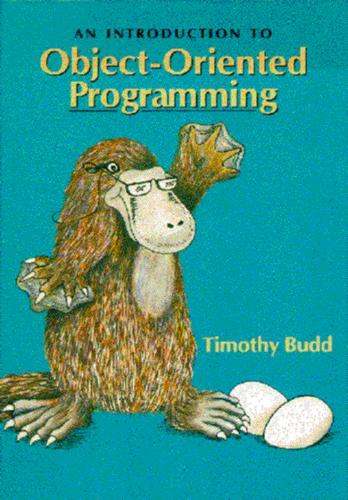
\includegraphics[height=0.8\textheight]{budd}
      \end{center}      
    \end{column}
    \begin{column}{0.5\linewidth}
      \begin{itemize}
      \item \href{http://web.engr.oregonstate.edu/~budd/}{Timothy A. Budd}
      \item Tres ediciones
      \item La segunda es asequible y está en biblioteca
      \end{itemize}
    \end{column}
  \end{columns}
\end{frame}

\begin{frame}{¿Por qué?}
  \begin{itemize}
  \item Dos conceptos esenciales en vuestra carrera:
    \begin{center}
      \larger
      \alert{Arquitectura}\\
      +\\
      \alert{Abstracción}\\
    \end{center}
    \pause
  \item Es como un \alert{campo de batalla en pequeño}
  \end{itemize}
\end{frame}
    
\begin{frame}{Evaluación}
  \begin{center}
    \begin{tabular}{ll}
      \alert{NT1} 15\% & Semana 5 o 6\\
      \alert{NT2} 45\% & Semana 15 o 16\\
      \multicolumn{2}{c}{\alert{Mínimo un 4}}\\
      \hline
      \alert{NE}\footnote{Ejercicios entregables en clase} 10\% & Semana 7 o 8\\
      \multicolumn{2}{c}{\alert{Mínimo un 3}}\\
      \hline
      \alert{NP}\footnote{Prácticas en casa, individuales o en pareja} 30\% & Semanas 9-11\\
      \multicolumn{2}{c}{\alert{Mínimo un 5}}\\
      \hline
      \alert{NPO}\footnote{Prácticas opcionales en casa casa, individuales o en pareja} 10\% & Semanas 12-15
    \end{tabular}
  \end{center}
\end{frame}

\tikzstyle{every picture}=[
    every matrix/.style={ampersand replacement=\&,column sep=1cm,row sep=1cm},
    mine/.style={draw,thick,rounded corners,fill=green!25},
    vendor/.style={draw,thick,rounded corners,fill=blue!25},
    tmp/.style={draw,thick,rounded corners,fill=yellow!25},
    product/.style={draw,thick,rounded corners,fill=red!25},
    data/.style={draw,thick,rounded corners,fill=yellow!25},
    process/.style={draw,thick,circle,fill=blue!25},
    to/.style={->,>=stealth',shorten >=1pt,semithick},
    every node/.style={align=center}]

\begin{frame}{¿Cómo funciona Java? i}
  \pause
  \smaller[2]
  \begin{center}
  \begin{tikzpicture}
    % Position the nodes using a matrix layout
    \matrix{
      \node (developer) {
\includegraphics[width=3em]{developer}};
      \& \node[process] (editor) {Editor\\(emacs)};
      \& \node[mine] (source) {\url{Hola.java}\\código fuente};\\
    };

    % Draw the arrows between the nodes and label them.
    \draw[to] (developer) -- (editor);
    \draw[to] (editor) -- (source);
  \end{tikzpicture}
  \pause
  \begin{tikzpicture}
    % Position the nodes using a matrix layout
    \matrix{
      \node[mine] (source) {\url{Hola.java}\\código fuente};
      \& \node[process] (javac) {Compilador\\(javac)};
      \& \node[product] (class) {\url{Hola.class}\\JVM bytecode};\\
    };

    % Draw the arrows between the nodes and label them.
    \draw[to] (source) -- (javac);
    \draw[to] (javac) -- (class);
  \end{tikzpicture}
  \pause
  \begin{tikzpicture}
    % Position the nodes using a matrix layout
    \matrix{
      \node[product] (class) {\url{Hola.class}\\JVM bytecode};
      \& \node[process] (java) {JVM\\(java)};
      \& \node[product] (resultado) {Resultado de\\la ejecución};\\
    };

    % Draw the arrows between the nodes and label them.
    \draw[to] (class) -- (java);
    \draw[to] (java) -- (resultado);
  \end{tikzpicture}
  \end{center}
\end{frame}

\begin{frame}[fragile]{\alert{\programar} ¿Cómo se crean objetos?}
  \smaller
  \begin{lstlisting}[escapeinside=!!]
public class Sesion02 {
  public static void main(String args[]) {
    !\alert<1>{A a}!;
    a !\alert<4>{=}! !\alert<2-3>{new A()}!;
  }
}
  \end{lstlisting}
  \vspace{-4ex}
  \begin{center}
    \only<1>{
\includegraphics[scale=0.25]{variable}}%
    \only<2>{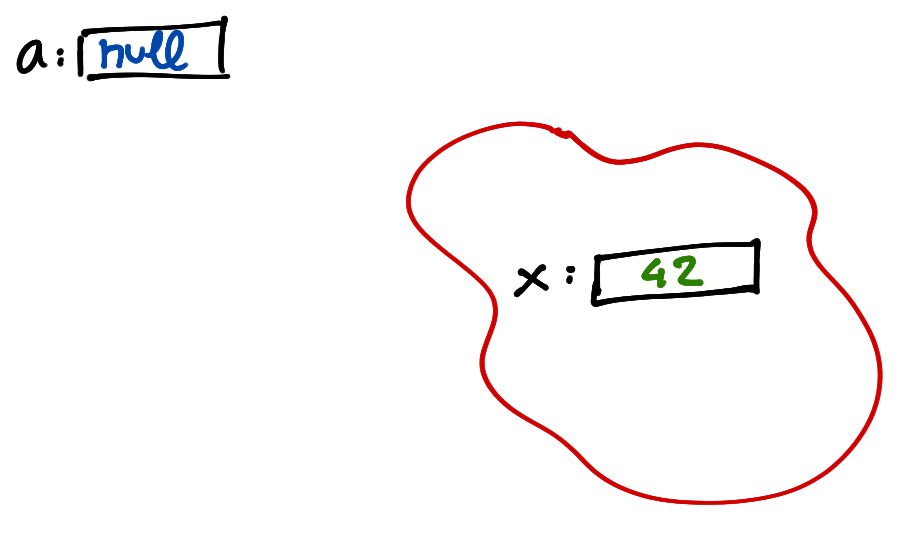
\includegraphics[scale=0.25]{objeto}}%
    \only<3>{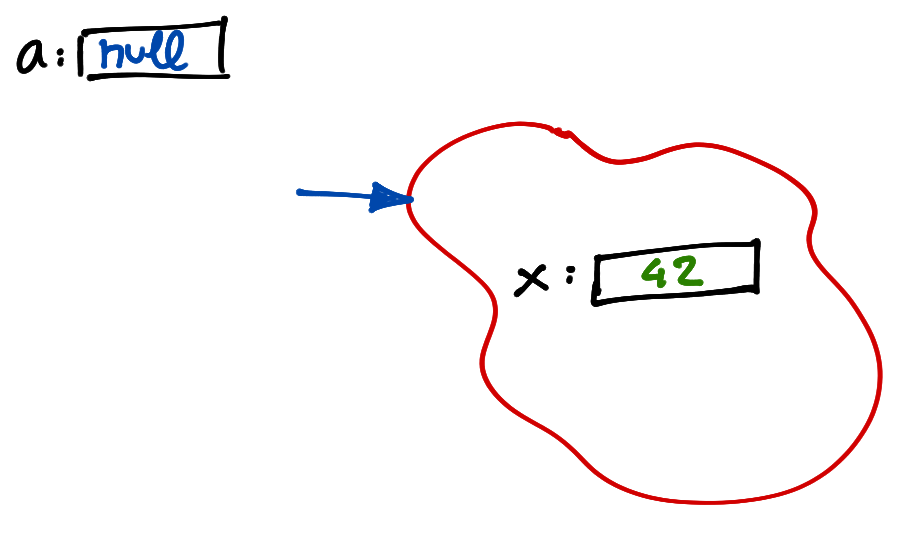
\includegraphics[scale=0.25]{new}}%
    \only<4>{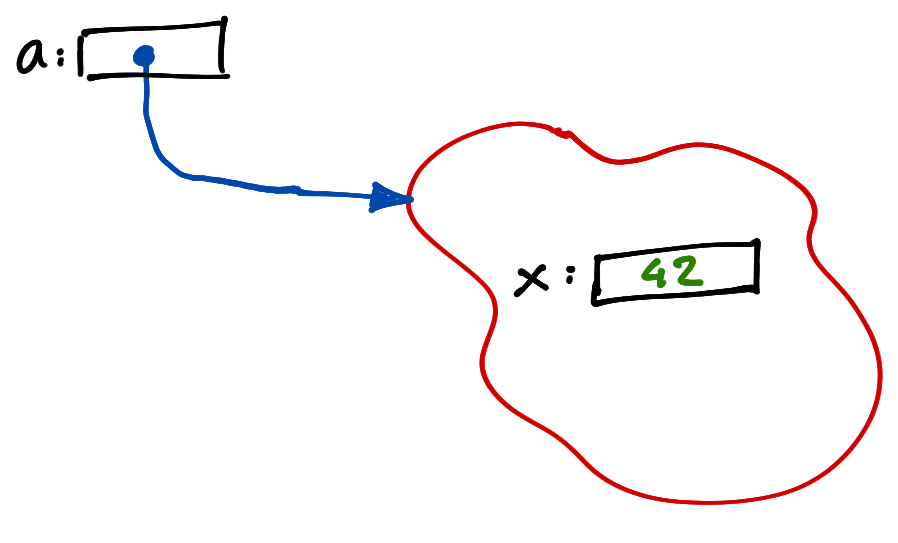
\includegraphics[scale=0.25]{assign}}
  \end{center}
\end{frame}

\end{document}

%%% Local Variables:
%%% mode: latex
%%% TeX-master: t
%%% End:
